  \let\negmedspace\undefined
\let\negthickspace\undefined
\documentclass[journal]{IEEEtran}
\usepackage[a5paper, margin=10mm, onecolumn]{geometry}
\usepackage{lmodern} % Ensure lmodern is loaded for pdflatex
\usepackage{tfrupee} % Include tfrupee package

\setlength{\headheight}{1cm} % Set the height of the header box
\setlength{\headsep}{0mm}     % Set the distance between the header box and the top of the text

\usepackage{gvv-book}
\usepackage{gvv}
\usepackage{cite}
\usepackage{amsmath,amssymb,amsfonts,amsthm}
\usepackage{algorithmic}
\usepackage{graphicx}
\usepackage{textcomp}
\usepackage{xcolor}
\usepackage{txfonts}
\usepackage{listings}
\usepackage{enumitem}
\usepackage{mathtools}
\usepackage{gensymb}
\usepackage{comment}
\usepackage[breaklinks=true]{hyperref}
\usepackage{tkz-euclide} 
\usepackage{listings}                                      
\def\inputGnumericTable{}                                 
\usepackage[latin1]{inputenc}                                
\usepackage{color}                                            
\usepackage{array}                                            
\usepackage{longtable}
\usepackage{multicol}
\usepackage{calc}                                             
\usepackage{multirow}                                         
\usepackage{hhline}                                           
\usepackage{ifthen}                                           
\usepackage{lscape}
\begin{document}

\bibliographystyle{IEEEtran}
\vspace{3cm}

\title{9.3.11}
\author{EE24BTECH11024 - G. Abhimanyu Koushik}
% \maketitle
% \newpage
% \bigskip
{\let\newpage\relax\maketitle}

\renewcommand{\thefigure}{\theenumi}
\renewcommand{\thetable}{\theenumi}
\setlength{\intextsep}{10pt} % Space between text and floats


\numberwithin{equation}{enumi}
\numberwithin{figure}{enumi}
\renewcommand{\thetable}{\theenumi}


\textbf{Question}:\newline
Solve the differential equation $\frac{d^2y}{dx^2} + 1 = 0$ with initial conditions $y\brak{0} = 0$ and $y^{\prime}\brak{0} = 0$
\newline
\textbf{Solution: }
\begin{table}[h!]    
  \centering
  \begin{tabular}[12pt]{ |c| c|}
    \hline
    \textbf{Variable} & \textbf{Description}\\
    \hline
    $n$ & Order of given differential equation\\
    \hline
    $a_i$ & Coeefficient of $i$th derivative of the function in the equation\\
    \hline
    $c$ & constant in the equation\\
    \hline
    $y^i$ & $i$th derivative of given function\\
    \hline
    $\vec{y}\brak{t}$ & $\myvec{c \\ y\brak{t} \\ y^\prime\brak{t} \\ \vdots \\ y^{n-1}\brak{t}}$\\
    \hline
    $h$ & stepsize, taken to be 0.001\\
    \hline
    $u\brak{x}$ & Unit step function\\
    \hline
    $k_0$ & proportionality constant\\
    \hline
    \end{tabular}

  \caption{Variables Used}
  \label{tab1.1.2.2}
\end{table}
\newline
Theoritical Solution:
\begin{align}
	\frac{d^2y}{dx^2} + 1 &= 0\\
	\frac{d^2y}{dx^2} &= -1\\
	\int_{}^{}\frac{d^2y}{dx^2}dx &= \int_{}^{}-1dx\\
	\frac{dy}{dx} &= -x+c_1\\
	\int_{}^{}\frac{dy}{dx}dx &= \int_{}^{}\brak{-x+c_1}dx\\
	y &= \frac{-x^2}{2}+{c_1}x+c_2
\end{align}
Substituting the initial conditions gives
\begin{align}
	y\brak{0} = 0 &\implies \frac{-0^2}{2}+{c_1}0+c_2 = 0\\
	c_2 &= 0\\
	y^{\prime}\brak{0} = 0 &\implies -0+c_1 = 0\\
	c_1 &= 0
\end{align}
The theoritical solution is 
\begin{align}
	f\brak{x} = \frac{-x^2}{2}
\end{align}
\newline
Computational Solution:\newline
Consider the given linear differential equation
\begin{align}
	a_{n}y^n + a_{n-1}y^{n-1} + \dots + a_{1}y^\prime + a_{0}y + c = 0
\end{align}
Then
\begin{align}
	y^{\prime}\brak{t} = \lim_{h\to 0}\frac{y\brak{t+h} - y\brak{t}}{h}\\
	y\brak{t+h} = y\brak{t} + hy^{\prime}\brak{t}
\end{align}
Similarly
\begin{align}
	y^{i}\brak{t+h} &= y^{i}\brak{t} + hy^{i+1}\brak{t}\\
	y^{n-1}\brak{t+h} &= y^{n-1}\brak{t} + hy^{n}\brak{t}\\
	y^{n-1}\brak{t+h} &= y^{n-1}\brak{t} + h\brak{-\frac{a_{n-1}}{a_n}y^{n-1}-\frac{a_{n-2}}{a_n}y^{n-2} - \dots -\frac{a_{0}}{a_n}y - \frac{c}{a_n}}
\end{align}
Where i ranges from 0 to $n-1$\\
\begin{align}
	\vec{y}\brak{t+h} = \vec{y}\brak{t} + \myvec{0 & 0 & 0 & 0 & \dots & 0 & 0\\ 0 & 0 & 1 & 0 & \dots & 0 & 0\\0 & 0 & 0 & 1 & \dots & 0 & 0\\\vdots & \vdots & \vdots & \vdots& \ddots & \vdots & \vdots\\
	0 & 0 & 0 & 0 & \dots & 0 & 1\\-\frac{1}{a_n} & -\frac{a_0}{a_n} & -\frac{a_1}{a_n} & -\frac{a_2}{a_n} & \dots & -\frac{a_{n-2}}{a_n} & -\frac{a_{n-1}}{a_n}}\brak{h\vec{y}\brak{t}}\\
	\vec{y}\brak{t+h} = \myvec{1 & 0 & 0 & 0 & \dots & 0 & 0\\ 0 & 1 & h & 0 & \dots & 0 & 0\\0 & 0 & 1 & h & \dots & 0 & 0\\\vdots & \vdots & \vdots & \vdots& \ddots & \vdots & \vdots\\
	0 & 0 & 0 & 0 & \dots & 1 & h\\-\frac{h}{a_n} & -\frac{a_0h}{a_n} & -\frac{a_1h}{a_n} & -\frac{a_2h}{a_n} & \dots & -\frac{a_{n-2}h}{a_n} & 1-\frac{a_{n-1}h}{a_n}}\brak{\vec{y}\brak{t}}
\end{align}
Discretizing the steps gives us
\begin{align}
	\vec{y}_{k+1} = \myvec{1 & 0 & 0 & 0 & \dots & 0 & 0\\ 0 & 1 & h & 0 & \dots & 0 & 0\\0 & 0 & 1 & h & \dots & 0 & 0\\\vdots & \vdots & \vdots & \vdots& \ddots & \vdots & \vdots\\
	0 & 0 & 0 & 0 & \dots & 1 & h\\-\frac{h}{a_n} & -\frac{a_0h}{a_n} & -\frac{a_1h}{a_n} & -\frac{a_2h}{a_n} & \dots & -\frac{a_{n-2}h}{a_n} & 1-\frac{a_{n-1}h}{a_n}}\brak{\vec{y}_{k}}
\end{align}
where $k$ ranges from 0 to number of data points with $y^{i}_0$ being the given initial condition.\\
For the given question\\
\begin{align}
	\vec{y}_{k+1} = \myvec{1 & 0 & 0\\ 0 & 1 & h\\ -h & 0 & 1}\vec{y}_k
\end{align}
Record the $y_k$ for 
\begin{align}
x_k =lowerbound+kh
\end{align}
and then plot the graph. The result will be as given below.
\begin{figure}[h!]
   \centering
   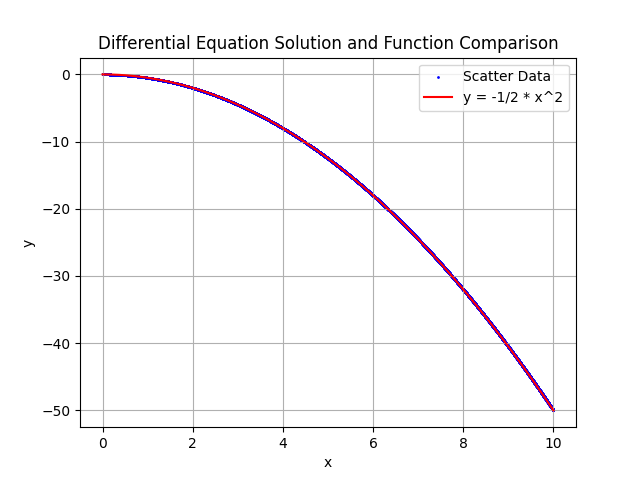
\includegraphics[width=\columnwidth]{figs/fig.png}
   \caption{Comparison between the Theoritical solution and Computational solution}
   \label{stemplot}
\end{figure}
\end{document}  
